

% Controls Chapter: Expanded and Enhanced
\subsection*{1. Introduction to Security Controls}
Effective threat modeling leads to the implementation of actionable security controls, which are technical, administrative, or physical safeguards designed to reduce risk by preventing, detecting, or responding to threats\cite{owasp,shostack2014}. Security controls must be carefully selected and integrated into the system architecture to address the specific risks identified during the threat modeling process.

\subsection*{2. Authentication and Authorization}
Authentication is the process of verifying user identity, while authorization determines access rights within the system\cite{owasp}. Robust authentication mechanisms, such as multi-factor authentication (MFA), help prevent unauthorized access. Strong password policies and secure storage solutions (e.g., bcrypt, Argon2) further enhance security. Role-based access control (RBAC) and the principle of least privilege ensure that users have only the permissions necessary to perform their tasks, reducing the risk of privilege escalation and insider threats.
\begin{itemize}
	\item Multi-factor authentication (MFA)
	\item Strong password policies and storage (bcrypt, Argon2)
	\item Role-based access control (RBAC)
	\item Principle of least privilege
\end{itemize}

\subsection*{3. Input Validation and Output Encoding}
Input validation ensures that only properly formed data enters the system, while output encoding prevents injection attacks such as cross-site scripting (XSS) and SQL injection\cite{owasp}. By validating all user input (preferably using whitelisting), employing output encoding, and using parameterized queries, organizations can significantly reduce the risk of exploitation.
\begin{itemize}
	\item Validate all user input (whitelisting preferred)
	\item Use output encoding to prevent XSS
	\item Employ parameterized queries to prevent SQL injection
\end{itemize}

\subsection*{4. Data Protection}
Data protection involves safeguarding sensitive information both at rest and in transit\cite{nist800154}. Encryption technologies such as TLS 1.3 for data in transit and AES-256 for data at rest are essential for maintaining confidentiality. Secure cookies (HTTPOnly, Secure, SameSite) and masking sensitive data in logs further reduce the risk of data leakage and unauthorized access.
\begin{itemize}
	\item Encrypt sensitive data in transit (TLS 1.3) and at rest (AES-256)
	\item Use secure cookies (HTTPOnly, Secure, SameSite)
	\item Mask sensitive data in logs
\end{itemize}

\subsection*{5. Monitoring, Logging, and Incident Response}
Monitoring is the process of detecting suspicious activity within the system, while incident response involves managing and mitigating security incidents\cite{uceda2015}. Centralized logging and monitoring solutions enable organizations to detect anomalies and respond quickly to potential threats. Setting up alerting for suspicious activity and developing a tested incident response plan are critical for minimizing the impact of security breaches.
\begin{itemize}
	\item Implement centralized logging and monitoring
	\item Set up alerting for suspicious activity
	\item Develop and test an incident response plan
\end{itemize}

\subsection*{6. Security Control Mapping Table}
The following table maps common security controls to specific threat categories, providing examples of tools and techniques used to mitigate each risk:
\begin{table}[H]
\centering
\begin{tabular}{|l|l|l|}
\hline
		extbf{Threat} & \textbf{Control} & \textbf{Tool/Technique} \\
\hline
Spoofing & MFA, strong authentication & Google Auth, Authy \\
Tampering & Input validation & OWASP ESAPI, ORM \\
Repudiation & Audit logs & ELK, Splunk \\
Info Disclosure & Encryption, access control & OpenSSL, GPG \\
DoS & Rate limiting, WAF & ModSecurity, Cloudflare \\
Privilege Escalation & RBAC, least privilege & IAM, sudoers \\
\hline
\end{tabular}
\caption{Mapping Security Controls to Threats\cite{owasp,shostack2014}}
\end{table}

\subsection*{7. Visual Mapping and Practical Guidance}
\begin{figure}[H]
	\centering
	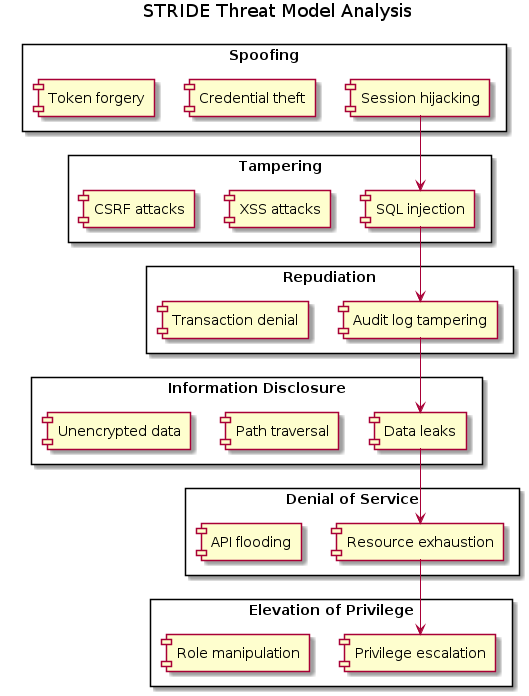
\includegraphics[width=0.7\textwidth]{images/stride-analysis}
	\caption{Security Controls Mapped to Threat Categories}
\end{figure}

\subsection*{8. Academic Perspective and Further Reading}
For deeper understanding, refer to:
\begin{itemize}
	\item Adam Shostack, "Threat Modeling: Designing for Security" (Wiley, 2014)
	\item Tony UcedaVélez and Marco M. Morana, "Risk Centric Threat Modeling" (Wiley, 2015)
	\item NIST SP 800-154: Guide to Data-Centric System Threat Modeling
	\item OWASP Threat Modeling Cheat Sheet
\end{itemize}
